\section{Datenmodellierung}
\label{kap:ERDiagramm}
MongoDB ist eine Dokument orientierte Datenbank. Dabei werden die Daten in JSON
ähnlichen Dokumenten verwaltet. Um das Entity-Relations Schema in die MongoDB
abbilden zu können, muss das Schema umgeformt werden. Dies ist auch bei
relationalen Datenbanken der Fall. In Abbildung \ref{fig:uni-db} ist das
ER-Schema der uni-DB abgebildet. Dies ist die Ausgangslage für unser Projekt.
MongoDB ist eine dokumentorientierte Datenbank. Dabei werden die Daten in Dokumenten verwaltet, die im JSON Format gespeichert werden. Das bedeutet, dass die Daten nicht relational
verwaltet werden. So kann zum Beispiel ein Tupel einer relationalen Datenbank
als Dokument in der dokumentorientierten Datenbank abgebildet werden. Die
Attribute und die dazugehörigen Werte werden dabei in Schlüssel-Wert Paare
abgebildet. 
\\\\
Unserem Projekt liegt das ER-Schema aus Abbildung \ref{fig:uni-db}
zugrunde.
Da MongoDB eine NoSQL und keine relationale Datenbank ist, kann das ER-Schema nicht direkt
in dieser Form in der Datenbank abgebildet werden. 

\begin{figure}[h] 
	\centering
		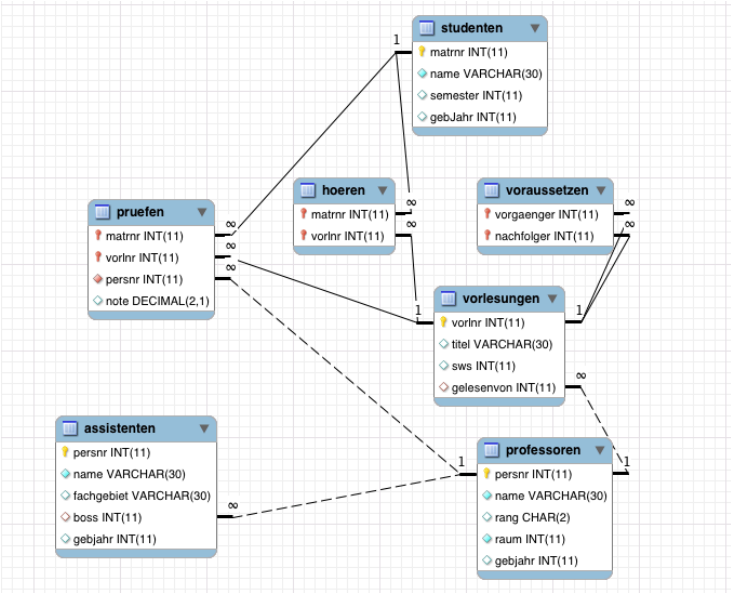
\includegraphics[width=1\textwidth]{./pictures/SQL-DB_ER_Diagramm_UNI-DB.png}
	\caption{ER-Diagramm zur Uni-DB \cite{Kaufmann2016}}
	\label{fig:uni-db}
\end{figure}

Das Schema der NoSQL Datenbank sieht wie folgt aus:
\begin{figure}[h] 
	\centering
		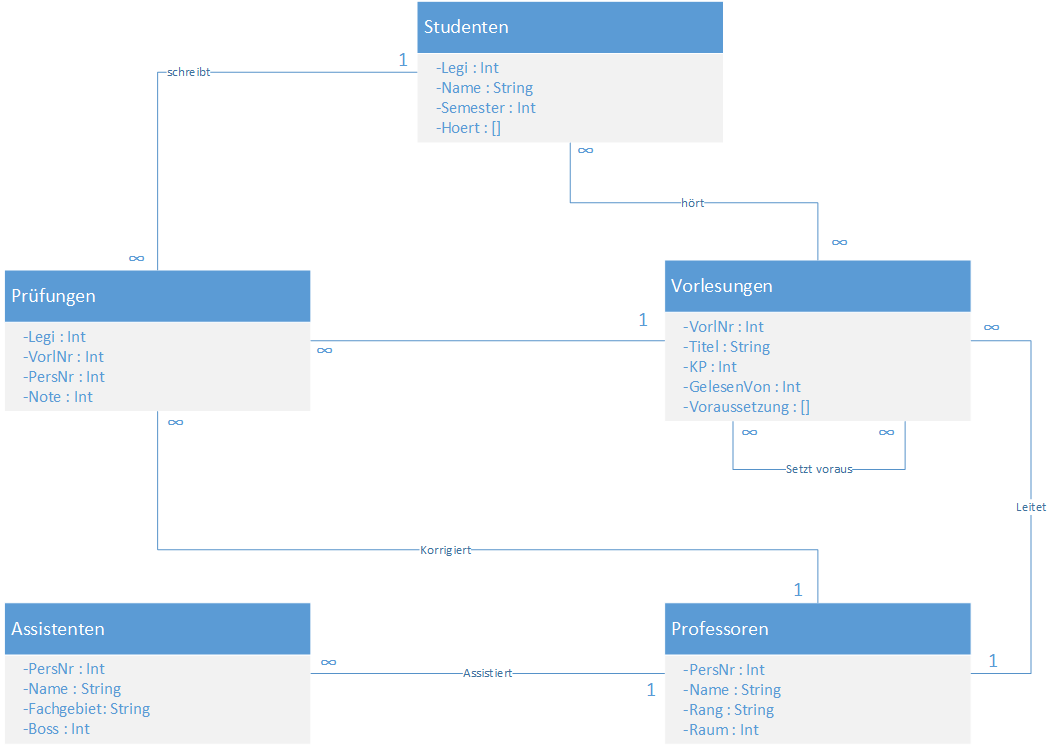
\includegraphics[width=1\textwidth]{./pictures/NoSQL-DB_ER_Diagramm_UNI-DB.png}
	\caption{ER-Diagramm zur Uni-DB}
	\label{fig:uni-db}
\end{figure}
Eine Collection der MongoDB entspricht der Tabelle in relationalen Datenbanken.
Das Dokument ist das Gegenstück zum Tupel. Die Attribute und die dazugehörigen
Werte werden in der MongoDB als Schlüssel-Wert Paare gespeichert.
Beziehungen werden in RDBMS als Fremdschlüssel abgebildet. In MongoDB 
können Relationen in Form von Werten eines bestimmten Keys gespeichert werden.
Komplex-Komplexe Beziehungen werden in RDBMS in eigene
Tabellen ausgelagert. Daraus entstehen dann zwei Einfach-Komplexe
Beziehungen. \\
Wie bereits erwähnt, muss das ER-Schema auch für die MongoDB umgeformt werden.
Starke Entitäten werden als Collections abgebildet, schwache Entitäten werden 
als Unterteil in das dazugehörige Dokument eingebettet.
Das Schema nach der Umformung ist in der Abbildung \ref{fig:uni-dbNoSQL}
ersichtlich.
\begin{figure}[h] 
	\centering
		
\includegraphics[width=1\textwidth]{./pictures/todo.jpg}
	\caption{MongoDB Schema zur Uni-DB }
	\label{fig:uni-dbNoSQL}
\end{figure}
Eine Komposition bedeutet, dass eine schwache Entität als Unterteil abgebildet
wird. Eine Aggregation bedeutet, dass starke Entität  als Referenz abgebildet
wird. In MongoDB wird die ID des Referenzierten Dokuments als Wert gepsiechert.
\\
Der folgenden JSON-Code zeigt ein Beispiel wie eine starke Entität
in MognoDB abgespeichert wird. Das Code-Beispiel zeigt das Dokument eines
Studenten. Die Vorlesungen, welcher dieser Student hört, werden im Werte Array
des Schlüssels Hören abgespeichert. Die Werte entsprechen dabei der ID der
Vorlesung.
 \begin{figure} [h]
	\begin{verbatim}
	{
		"Legi": 25403,
		"Name" : "Jonas",
		"Semester" : 12,
		"Hören" : [5032, 1910],
	}
	\end{verbatim}
	\label{cod:vorlesung}
\end{figure}


